\section{Introduction}
\label{sec-introduction}

%Define the problem and the goal of the project
%Explain why the problem is important
%Summarize your approach and key results
%Outline the rest of the paper

Since the advent of the Internet, computing devices have become not only more
prolific but also more varied - encompassing not only high performance
clusters but also general purpose computers and mobile systems.  Moreover, the
assumptions made about the security model of a system have changed drastically;
users can no longer be trusted, and devices have the potential to interact with
unknown and possibly untrustworthy hosts while communicating sensitive
information. For example, the boom in smartphones has caused a secondary
explosion in the mobile application industry, allowing users to log in to
various trusted systems (e.g. bank accounts, medical records and shopping
accounts) remotely.  The sudden increase in connectivity exposes users to
adversaries that may attempt to leverage these interactions in order to obtain
confidential information or disrupt the use of services or applications.

In response to these changes, there has been an increasing effort in developing
trusted computing platforms augmented with specialized hardware modules that
provide security features such as authentication and decryption/encryption. One
such security feature that remains a focus in trusted computing research is
protecting off-chip memory. One key component of protecting off-chip memory is
maintaining confidentiality of private data. Challenges in designing memory
protection mechanisms involves providing encryption primitives at a low cost
(money, area, power and design complexity), high throughput and low latency
without compromising security. Current work also focuses on memory protection
schemes for general purpose and high performance computing systems. The domain
of memory protection in the mobile and embedded computing domains is relatively
less studied and poses interesting challenges. Mobile and embedded devices
often operate under strict power and area constraints. Providing secure memory
protection while following the prescribed power and area constraints as well as
maintaining performance of the computing devices is an ongoing challenge.

According to Hollis \cite{hollis} there are two main source of power
consumption when driving I/O:

\paragraph{Dynamic A/C Power} Dynamic A/C power consumption from charging and
discharging capacitances (e.g. electrostatic discharge devices, driver output
capacitance, receiver input capacitance and the channel itself), is possibly
the dominant and most universal form of I/O power consumption. However, once
the capacitances have reached steady state, the dynamic a/c power consumption
is negligible. For the purposes of our study we assume that all device
capacitances are already in steady state - simplifying our model as we no
longer have to consider dynamic a/c power consumption.

\paragraph{Link Termination} The second most common source of I/O power
consumption is link termination schemes. Intuitively, when the driver
outputs a signal which is then received by the I/O device, a significant
portion of the signal is reflected back to the driver itself. Consequently, the
driver has to not only power the desired signal but also overcome the signal
reflections.  This incurs a significant power overhead. Past research in the
context of link termination schemes has focused on developing more efficient
DDR chip topologies to reduce signal reflections. For example, in Figure
\ref{dram-chips} illustrates the DDR2 and DDR3 DDR chip topologies. As driving
frequencies for DDR3 increased, memory architects adopted the fly-by network
topology which greatly reduces signal reflections and improves On-Die
Termination (ODT).

\begin{figure}[!htb]
  \centering
  \begin{subfigure}[b]{0.4\textwidth}
    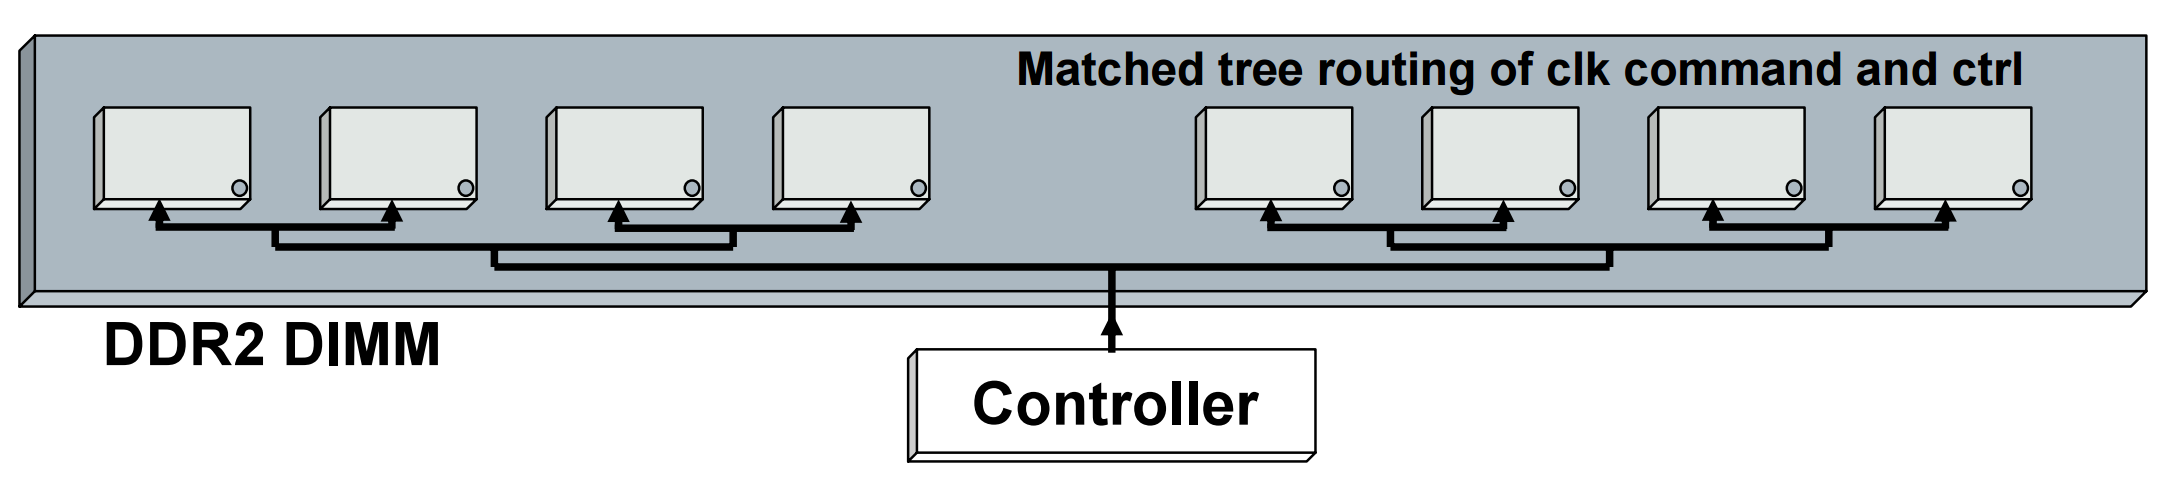
\includegraphics[width=\textwidth]{figs/ddr2-topology}
    \caption{Example DDR2 DRAM chip topology}
    \label{fig:ddr2-chips}
  \end{subfigure}

  \begin{subfigure}[b]{0.4\textwidth}
    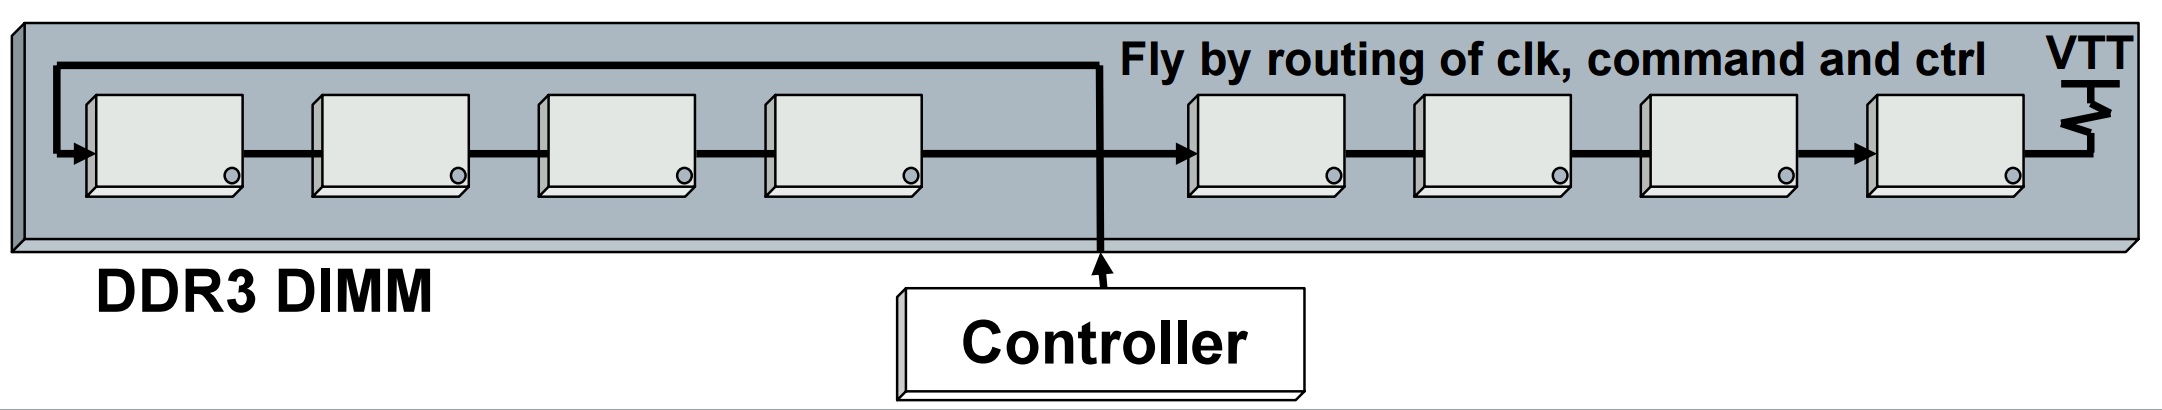
\includegraphics[width=\textwidth]{figs/ddr3-topology}
    \caption{Example DDR3 DRAM chip topology}
    \label{fig:ddr3-chips}
  \end{subfigure}
  \caption{Representative DRAM chip topologies for DDR2 and DDR3 memory
  technologies taken from \cite{ddr-design}}
  \label{dram-chips}
\end{figure}

Though existing DDR3 memory technologies implement more efficient DRAM chip
topologies to reduce signal reflections, ODT is still a prominent source of
power consumption. Memory architects are looking at more efficient read/write
schemes such as Data Bus Inversion (DBI) for further improving ODT power
consumption for DDR4. Our study focuses on using first order models for DBI
developed by Hollis \cite{hollis} in the context of memory encryption to
simulate the power overhead of secure memory encryption. Generally, our results
so that memory encryption does indeed incur a significant power overhead and
that DBI-DC and AC values for is relatively consistent across MiBench
applications.

The rest of this paper is organized as follows: Section~\ref{sec-problem}
outlines our general project goals and outlines the memory encryption model
used, Section~\ref{sec-methodology} outlines the high level model and
experimental setup for our study, Section~\ref{sec-evaluation} analyzes our
results and data, Section~\ref{sec-group-dynamics} reviews our group dynamic's
and work distribution, Section~\ref{sec-related} reviews related work in
relation to power consumption of secure memory encryption and
Section~\ref{sec-conclusions} concludes the paper with final remarks and future
work.
